\documentclass[border=6pt]{standalone}
% Shared preamble for web figures.  Each figure is a standalone .tex that
% \input's this file; scripts/make-figures.sh turns it into an SVG.
% Handouts pull the same file with \fig{Unit_X/<name>}.
\usepackage[T1]{fontenc}
\usepackage{helvet}
\renewcommand{\familydefault}{\sfdefault}
\renewcommand{\ttdefault}{pcr}  % Courier: a real Type 1 typewriter font
\usepackage{amsmath}
\usepackage{tikz}
\usetikzlibrary{arrows.meta,positioning,calc,shapes.symbols,shapes.geometric}

% Who makes the rules is the point of most diagrams in this book, so the
% colors mean the same thing everywhere: blue is a person, orange is the
% computer, green is an answer, pink is the human brain.
\definecolor{person}{HTML}{2C6FAE}
\definecolor{machine}{HTML}{D35400}
\definecolor{result}{HTML}{1E8449}
\definecolor{brainpink}{HTML}{C2185B}
\definecolor{ink}{HTML}{2C3E50}

\tikzset{
  doodle/.style={line width=1.5pt, line cap=round, line join=round, draw=ink},
  box/.style={draw, rounded corners=5pt, line width=1.1pt, align=center,
              inner sep=7pt, minimum height=1.0cm, font=\small},
  personbox/.style={box, draw=person, fill=person!10},
  machinebox/.style={box, draw=machine, fill=machine!10},
  resultbox/.style={box, draw=result, fill=result!10},
  plainbox/.style={box, draw=ink!70, fill=ink!4},
  flow/.style={-{Stealth[length=8pt]}, line width=1.4pt, draw=ink},
}

% A person (blue) and a robot head (orange) as small icons.
% \personicon{x}{y}{scale}   \roboticon{x}{y}{scale}
\newcommand{\personicon}[3]{%
  \begin{scope}[shift={(#1,#2)}, scale=#3]
    \fill[person] (0,0.62) circle (0.28);
    \fill[person, rounded corners=6pt] (-0.42,-0.55) rectangle (0.42,0.28);
  \end{scope}}
\newcommand{\roboticon}[3]{%
  \begin{scope}[shift={(#1,#2)}, scale=#3]
    \draw[machine, line width=1.2pt] (0,0.5) -- (0,0.72);
    \fill[machine] (0,0.78) circle (0.08);
    \draw[machine, line width=1.4pt, fill=machine!12, rounded corners=4pt] (-0.5,-0.45) rectangle (0.5,0.5);
    \fill[ink] (-0.2,0.12) circle (0.08);
    \fill[ink] (0.2,0.12) circle (0.08);
    \draw[ink, line width=1pt] (-0.22,-0.22) -- (0.22,-0.22);
  \end{scope}}

\begin{document}
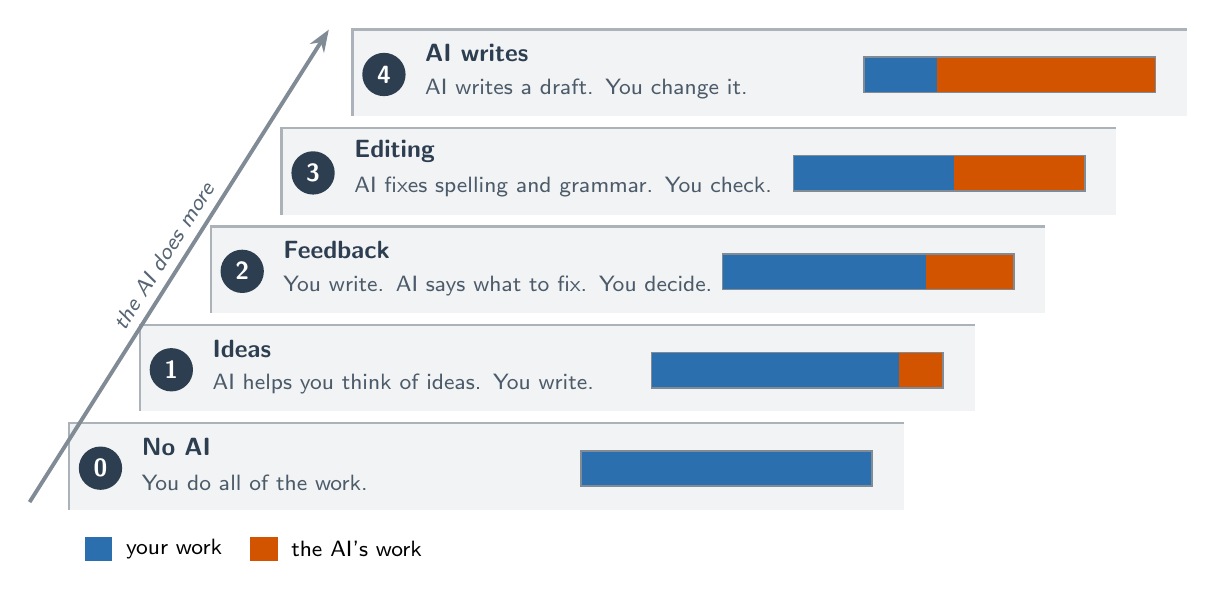
\begin{tikzpicture}[
  lbl/.style={font=\small\bfseries, text=ink, anchor=west},
  sub/.style={font=\footnotesize, text=ink!85, anchor=west, text width=5.5cm},
]
% The AI use ladder: each step up, the AI does more of the work.
% Bar: blue = the student's work, orange = the AI's work.
\foreach \k/\you/\name/\what in {
  0/1.0/No AI/You do all of the work.,
  1/0.85/Ideas/AI helps you think of ideas. You write.,
  2/0.7/Feedback/You write. AI says what to fix. You decide.,
  3/0.55/Editing/AI fixes spelling and grammar. You check.,
  4/0.25/AI writes/AI writes a draft. You change it.} {
  \pgfmathsetmacro{\y}{\k*1.25}
  \pgfmathsetmacro{\x}{\k*0.9}
  % step
  \fill[ink!6] (\x,\y-0.5) rectangle (\x+10.6,\y+0.6);
  \draw[ink!40, line width=0.8pt] (\x,\y-0.5) -- (\x,\y+0.6) -- (\x+10.6,\y+0.6);
  \node[circle, fill=ink, text=white, font=\small\bfseries, inner sep=2pt, minimum size=0.55cm] at (\x+0.4,\y+0.03) {\k};
  \node[lbl] at (\x+0.8,\y+0.3) {\name};
  \node[sub] at (\x+0.8,\y-0.15) {\what};
  % work bar
  \fill[person] (\x+6.5,\y-0.2) rectangle (\x+6.5+3.7*\you,\y+0.25);
  \fill[machine] (\x+6.5+3.7*\you,\y-0.2) rectangle (\x+10.2,\y+0.25);
  \draw[ink!60, line width=0.6pt] (\x+6.5,\y-0.2) rectangle (\x+10.2,\y+0.25);
}
\fill[person] (0.2,-1.15) rectangle (0.55,-0.85); \node[font=\footnotesize, anchor=west] at (0.6,-1.0) {your work};
\fill[machine] (2.3,-1.15) rectangle (2.65,-0.85); \node[font=\footnotesize, anchor=west] at (2.7,-1.0) {the AI's work};
\draw[flow, draw=ink!60] (-0.5,-0.4) -- (3.3,5.6) node[pos=0.5, sloped, above, font=\footnotesize\itshape, text=ink!80] {the AI does more};
\end{tikzpicture}
\end{document}
